\chapter{Design and materials}
In this section we will discuss the design of our mechanical, electronic, and software systems and the materials used.

\section{Block Diagram}
Below is a block diagram showing the general control flow of the entire system and all its components.

\begin{figure}[h]
	\centering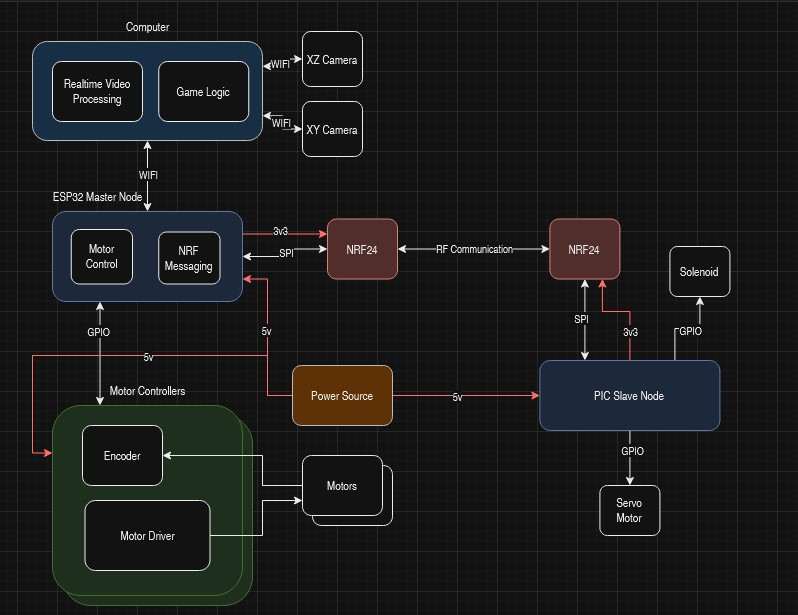
\includegraphics[height=3cm]{./images/blockdiagram}
	\caption{System Design Block Diagram}
\end{figure}

\section{Electronic Components and Controllers}
The system mainly relies on 2 mobile phones which are used for collecting the position information of the ping pong ball with 3 degrees of freedom. The mobile phones are configured with an app to act as IP cameras, which are then accessed over Wi-Fi on the control device, which is a laptop running our software.

The ESP32 microcontroller is connected to 3 stepper motor driver modules (DRV8825), which are in turn connected to 3 R.T.A. bipolar stepper motors which control the gantry. The ESP32 acts as a master to a PIC18F, though a connected radio frequency communication module (NRF24), which is used to transmit data to another NRF24 module, connected to the PIC18F slave microcontroller. This data consists of information on when to "fire" the racket to hit the ball, by activating the optcoupled 12v solenoid, and information on what angle the racket should be at, by controlling the 6v servo motor controlling the racket.

\begin{figure}[h]
	\centering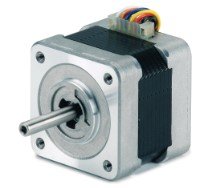
\includegraphics[height=3cm]{./images/steppermotor}
	\caption{Stepper Motor Used}
\end{figure}

\section{Software Design}
The main software which controls the system is ran a separate computer, due to the speed constraints of small microcontrollers. The code connects to the IP camera phones, reads the streamed video data, and process it using ball detection algorithms to determine the position of the ping pong ball in 3D space. The software sends a requested gantry position, a requested racket orientation, and when the racket should "fire" over Wi-Fi to the ESP32 microcontroller, which then sends this data over radio using the NRF24 to the PIC18F.

The software additionally maintains the game state through a simplified ruleset, allowing the score and current ball position to be visualized in real time. The software determines the ball's position and additionally applies a predictive model to determine where the gantry should move to.


\section{Printed Circuit Boards}

Our design additionally consists of 2 Printed Circuit Boards (PCBs), one for each used microcontroller. The first PCB designed is for the PIC18F slave microcontroller. It contains connections for the solenoid, and its control circuit which consists of an optocoupler and a Darlington NPN bipolar transistor (TIP120). It also cor ontains connections for the servo motor and its control circuit which is a simple MOSFET transistor circuit. It also contains connections for the NRF24 module.

\begin{figure}[h]
	\centering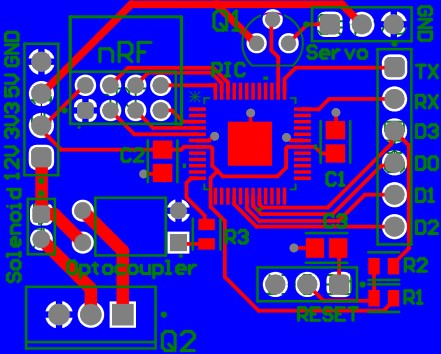
\includegraphics[height=3cm]{./images/picpcb}
	\caption{PIC18F PCB Design}
\end{figure}

The second designed PCB is for the ESP32 master controller. This PCB consists of headers for the ESP32 controller itself, and headers for each of the DRV8825 modules. It has a switch for on board adjustment of the drivers' control pins. It also contains connections for the NRF24 module.

\begin{figure}[h]
	\centering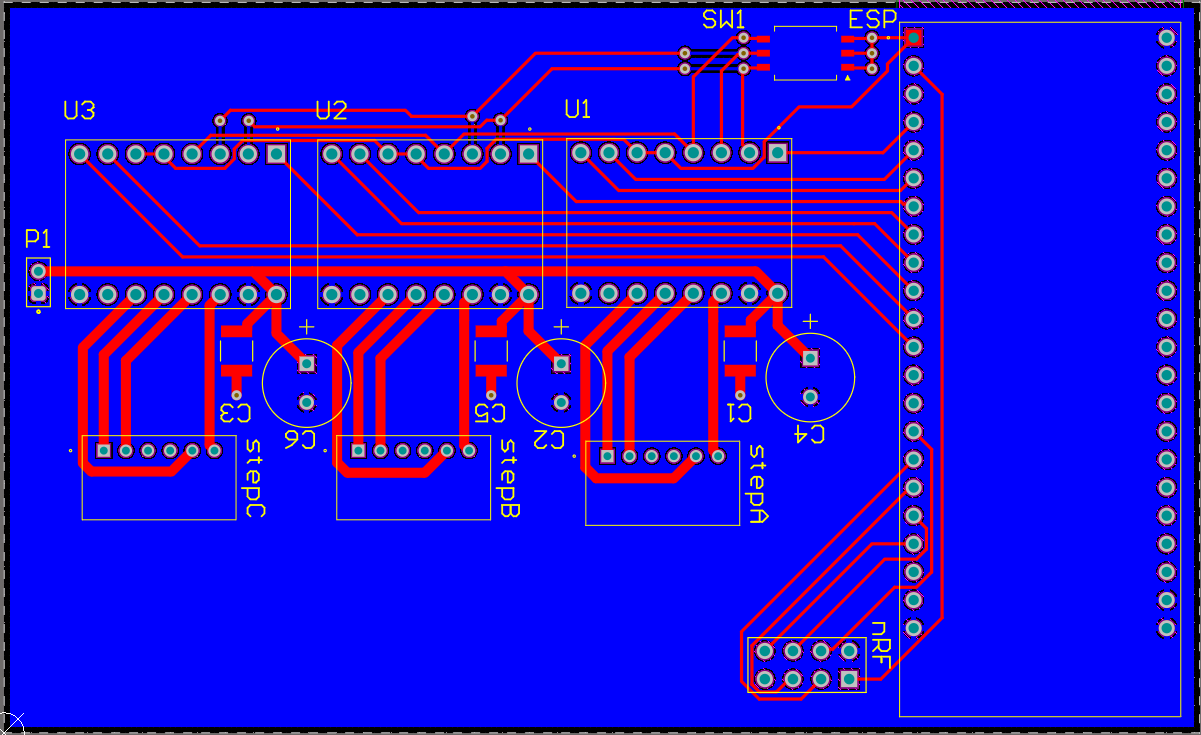
\includegraphics[height=3cm]{./images/esppcb}
	\caption{ESP32 PCB Design}
\end{figure}

\section{Bill of Materials}

\begin{center}
\begin{tabular}{|l|c|c|c|}
 \hline
Item & Amount & Price (\texteuro) \\
 \hline\hline
 MDF (60x30) & - & 2 \\ 
 \hline
 3D Printed Parts & 100g & 10\\
 \hline
 Timing Belt & - & 4.5\\
 \hline
 Servo Motor & 1 & 3.5 \\
 \hline
 Solenoid & 1 & 6.9 \\ 
 \hline
 ESP32 & 1 & 6.9 \\
 \hline
 PIC18F & 1 & 2.4 \\
 \hline
 NRF24 & 2 & 6.68 \\
 \hline
 Stepper Motor & 3 & - \\
 \hline
 Stepper Driver DRV8825 & 3 & 13.5 \\
 \hline
 Optocoupler & 1 & - \\
 \hline
 Transistors & - & - \\
 \hline
 Resistors & - & - \\
 \hline
 Capacitors & - & - \\
 \hline
\end{tabular}
\end{center}